\documentclass[a4paper,10.5pt,twocolumn]{ltjsarticle}

\usepackage{luatexja}
\usepackage{amsmath,amssymb}
\usepackage{graphicx}
\usepackage{booktabs}
\usepackage[hidelinks]{hyperref}
\usepackage[top=20truemm,bottom=22truemm,left=18truemm,right=18truemm,columnsep=8mm]{geometry}

\ltjsetparameter{jacharrange={-2}}
\pagestyle{empty}

% ---- 参考文献番号を [1] 形式に ----
\makeatletter
\renewcommand{\@biblabel}[1]{[#1]}
\makeatother

\begin{document}

\twocolumn[
\begin{center}
{\LARGE\bfseries AR技術を用いた大学キャンパスナビゲーションシステムの開発}\\*
\vspace{3mm}
{\large Development of an AR-based Campus Navigation System for University Use}\\*
\vspace{6mm}
{\normalsize 生亀太郎\ \ 生亀花子\quad 専修大学 ネットワーク情報学部}\\*
\vspace{2mm}
{\normalsize Taro Ikugame, Hanako Ikugame\quad Faculty of Network and Information, Senshu University}\\*
\vspace{8mm}
\end{center}
]

\section{まえがき}

専修大学生田キャンパスは複数の号館が渡り廊下や連絡通路で入り組んで接続されており，初めて訪れる新入生・教職員・来訪者が目的の教室や施設に迷わずたどり着くことは容易ではない。従来設置されている紙媒体の案内図や固定式の案内板では，現在地から目的地までの動的な経路提示ができないという課題がある。

そこで我々は，スマートフォンのブラウザから利用できるAR対応キャンパスナビゲーションWebアプリケーション「IKU NAVI」を開発した。本プロジェクトの基本方針は，専用アプリの導入や高精度な自己位置推定を要する本格的なARではなく，\textbf{経路写真に矢印を合成する簡易なARから着手し，段階的に発展させる}ことである。本稿では，屋内外を統合した経路探索の設計と，2段階に分けたAR実装，および大学規模のサービスとして低コストに運用するためのインフラ構成について報告する。

\section{システム設計}

\subsection{屋内外統合グラフによる経路探索}

建物内のノードには「建物ID$\times$100{,}000＋ローカルID」，屋外ノードには「ローカルID＋9{,}000{,}000」のグローバルIDを付与し，キャンパス全体を単一のグラフとして扱う。各建物のローカル座標は，2点のアンカー座標から回転角$\theta$と平行移動量$(t_x,t_y)$を最小二乗的に算出し，
\begin{align}
X_{g} &= \cos\theta\, X_{l} - \sin\theta\, Y_{l} + t_x,\\
Y_{g} &= \sin\theta\, X_{l} + \cos\theta\, Y_{l} + t_y
\end{align}
によりキャンパス全体の座標系へ変換する。エッジには通路・階段・エレベーター・エスカレーター（上り／下り一方向）・建物出入口の6種別を定義し，エスカレーターの一方向制約や車椅子利用者向けのエレベーター除外オプションをグラフ構造として表現した。教室名はノードではなくエッジの属性として管理し，最短経路探索（NetworkXの双方向Dijkstra法）では出発・目的の教室に対応するエッジの両端ノードを候補として全組み合わせを評価することで，複数出入口を持つ教室にも対応した。

\subsection{GPSによる屋外シームレス連携}

スマートフォンのGPSで取得した現在地は，Haversine距離により最寄りの屋外ノードへスナップし，出発ノードとして経路探索APIへ渡す。GPS精度が30mを超える場合は案内板の参照を促す警告を表示し，最寄りノードまでの距離が500mを超える場合はキャンパス外にいると判断して自動出発地点への採用を行わない仕組みとした。

\begin{figure}[t]
\centering
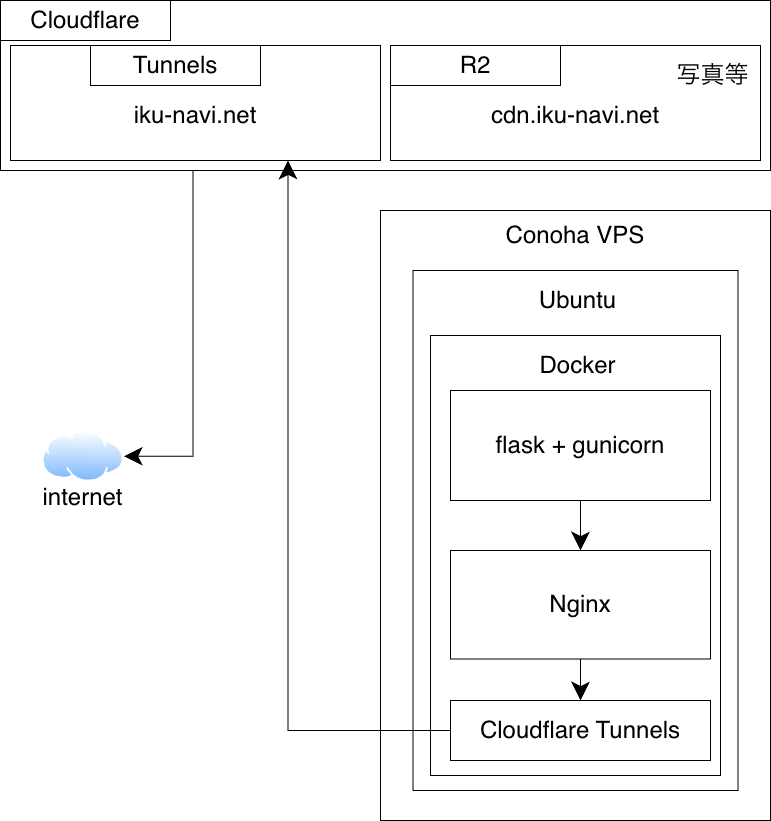
\includegraphics[width=0.85\linewidth]{../images/プロジェクト構成図.png}
\caption{システム全体構成図}
\label{fig:arch}
\end{figure}

\section{2段階のAR実装}

ナビゲーション中のAR表示は，現在のステップのノードが屋内・屋外いずれに属するかで自動的に切り替わる（図\ref{fig:arch}）。

\textbf{屋内AR：}経路確定直後にCDN配信の経路写真（両端ノード対応のJPEG）を全ステップ分先読みし，進行方向（左・右・直進，折れ角45°以内を直進とみなす）を示す矢印画像を重畳表示する。画像はDOM上に生成済みのため，ステップ移動時は表示クラスの付け替えのみで遅延なく切り替わる。

\textbf{屋外AR：}Three.jsによるWebGL描画とリアカメラ映像を合成する。緯度経度を基準点からの相対距離に変換してENU座標系にマッピングし，GPS更新のたびに世界座標を移動させることで現在地を原点とする相対配置を維持する。端末の方位センサーは，Android Chromeの絶対方位イベント，iOS Safariのコンパス方位，その他Androidの相対方位イベントの順にフォールバックして取得する。

\textbf{プライバシー・電力への配慮：}カメラはルートに屋外AR区間が含まれる場合のみ起動し，屋内のみの経路では起動しない。GPSの継続取得も屋外AR表示時にのみ有効化し，以降の区間に屋外ARが不要になった時点でストリームを解放することで，バッテリー消費と権限利用を必要最小限に抑えた。

\section{インフラと運用}

本番環境はConoHa VPS（平常時メモリ2GB）上のDocker Swarmで構築し，Flaskによる経路探索API・アクセスカウンター・監視基盤（Prometheus/Grafana）をコンテナとして稼働させている。学園祭等のイベント時には4GBサーバーをSwarmワーカーとして追加し，APIのレプリカ数を2から4へ拡張することで同時接続増に対応する。外部公開はCloudflare Tunnel経由に限定してポート開放を不要にし，静的コンテンツはCloudflare Pagesから配信することでVPS側の負荷を軽減した。表\ref{tab:req}に主な非機能要件を示す。

\begin{table}[t]
\centering
\small
\caption{主な非機能要件}
\label{tab:req}
\begin{tabular}{ll}
\toprule
項目 & 目標値 \\
\midrule
同時接続数 & 通常30人以下／ピーク100人以下 \\
APIレスポンス & 2秒以内 \\
目標稼働率 & 70\%以上 \\
\bottomrule
\end{tabular}
\end{table}

2026年2月の開発開始以降，データ設計・経路探索・フロントエンド・インフラを内製し，本稿執筆時点で本番運用中である。データ品質担保のため，全教室ペアの経路を並列探索して想定外の迂回やフロア逆走を自動検出するツールを独自開発し，スプレッドシート経由でのデータ更新運用と組み合わせて継続的なデータ整備を行っている。

\section{むすび}

本稿では，屋内外統合グラフに基づく経路探索と，写真合成型の屋内ARおよびThree.js/GPSによる屋外ARを組み合わせた大学向けナビゲーションシステムの設計・実装について報告した。今後は未整備建物のフロアマップ拡充，経路探索ロジックの自動テスト化，経路計算のブラウザ側移行による静的配信化，および屋内ARの高度化に取り組む予定である。

\begin{thebibliography}{9}
\bibitem{iku-navi} IKU NAVI, \url{https://iku-navi.net/}
\end{thebibliography}

\end{document}
